% Surface code on IQM Emerald -- hackathon presentation
% Build:  python presentation/build_data.py   (from the repo root)
%         cd presentation && latexmk -pdf main.tex
\documentclass[aspectratio=169,11pt]{beamer}
\usepackage[T1]{fontenc}
\usepackage[utf8]{inputenc}
\usepackage{booktabs}
\usepackage{siunitx}
\usepackage{tikz}
\usepackage{pgfplots}
\usepackage{pgfplotstable}
\pgfplotsset{compat=1.18}
\usetikzlibrary{arrows.meta,positioning,calc,fit,backgrounds,shapes.geometric}
\usepgfplotslibrary{groupplots}

% ── colours: deck + validated categorical chart palette ─────────────────────
\definecolor{ink}{HTML}{13202E}
\definecolor{soft}{HTML}{475569}
\definecolor{paper}{HTML}{F6F5F0}
\definecolor{panel}{HTML}{E9E7DF}
\definecolor{accent}{HTML}{C4621B}
\definecolor{cblue}{HTML}{2A78D6}
\definecolor{corange}{HTML}{EB6834}
\definecolor{caqua}{HTML}{1BAF7A}
\definecolor{cyellow}{HTML}{EDA100}
\definecolor{cgray}{HTML}{8A8780}
\definecolor{gridc}{HTML}{DDD9CE}
\colorlet{zstab}{cblue!22}
\colorlet{xstab}{corange!22}

\setbeamercolor{background canvas}{bg=paper}
\setbeamercolor{normal text}{fg=ink}
\setbeamercolor{frametitle}{fg=ink}
\setbeamercolor{title}{fg=ink}
\setbeamercolor{structure}{fg=accent}
\setbeamercolor{itemize item}{fg=accent}
\setbeamerfont{frametitle}{series=\bfseries,size=\Large}
\setbeamertemplate{navigation symbols}{}
\setbeamertemplate{itemize item}{\small\raise1.25pt\hbox{\color{accent}$\blacktriangleright$}}
\setbeamertemplate{footline}{\hfill\color{soft}\scriptsize\insertframenumber\ /\ \inserttotalframenumber\hspace*{1.2em}\vspace*{0.8em}}
\setbeamertemplate{frametitle}{\vspace*{0.6em}\insertframetitle\par\vspace*{-0.2em}%
  {\color{accent}\rule{2.2em}{2pt}}}

\makeatletter\newcommand{\tableinput}[1]{\@@input #1 }\makeatother
\newcommand{\eyebrow}[1]{{\color{accent}\scriptsize\bfseries\MakeUppercase{#1}}\par\smallskip}
\newcommand{\bignum}[2]{\begin{minipage}[t]{\linewidth}\centering{\color{cblue}\Huge\bfseries #1}\\[2pt]{\color{soft}\footnotesize #2}\end{minipage}}

\pgfplotsset{
  deck/.style={
    width=\linewidth, height=0.62\textheight, axis lines*=left,
    grid=major, major grid style={gridc}, axis line style={gridc},
    tick label style={color=soft,font=\scriptsize}, label style={color=soft,font=\footnotesize},
    legend style={draw=none,fill=none,font=\scriptsize,text=ink}, legend cell align=left,
    every axis plot/.append style={line width=1.4pt, mark size=2.4pt},
  }}

\title{A distance-3 surface code on IQM Emerald}
\subtitle{No mid-circuit reset, zero SWAPs, a characterized noise model and four decoders on 400\,000 hardware shots}
\author{[Team name] \quad [Names]}
\date{IQM QEC challenge}

\begin{document}

% ─────────────────────────────────────────────────────────────────────────────
{\setbeamercolor{background canvas}{bg=ink}\setbeamercolor{normal text}{fg=paper}
 \setbeamercolor{title}{fg=paper}\setbeamercolor{subtitle}{fg=panel}\setbeamercolor{author}{fg=panel}
\begin{frame}[plain]
  \color{paper}\vfill
  {\color{accent!80!white}\scriptsize\bfseries IQM QEC CHALLENGE \textperiodcentered\ MEMORY EXPERIMENT}\par\medskip
  {\Huge\bfseries A distance-3 surface code\\[2pt] on IQM Emerald}\par\bigskip
  {\large\color{panel} No mid-circuit reset, zero SWAPs, a characterized noise model\\ and four decoders, on 400\,000 hardware shots.}\par\vfill
  {\small\color{panel} [Team name] \textperiodcentered\ [Names]}
  \vspace*{1em}
\end{frame}}
% Notes: we built the full memory experiment, ran it on Emerald, and the syndromes told us what calibration did not.

% ─────────────────────────────────────────────────────────────────────────────
\begin{frame}{From a Stim circuit to a logical error rate}
\eyebrow{The pipeline}
\centering
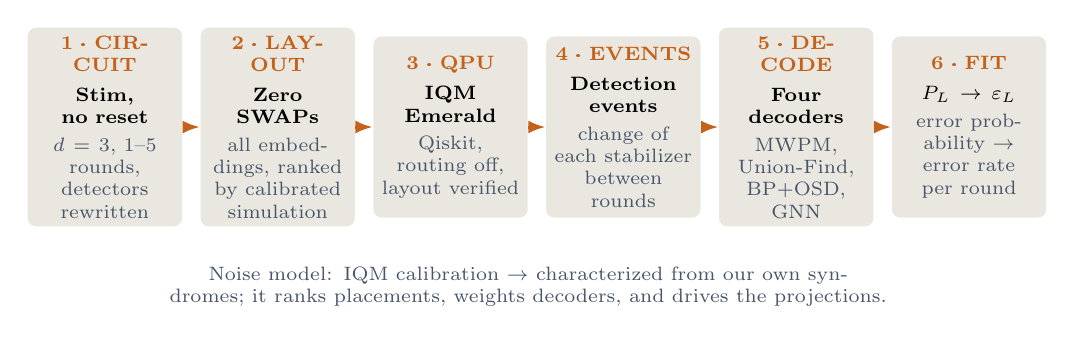
\begin{tikzpicture}[
  box/.style={draw=none,fill=panel,rounded corners=3pt,minimum width=1.9cm,minimum height=2.3cm,
              align=center,font=\scriptsize,text width=1.75cm,inner sep=3pt},
  arr/.style={-{Latex[length=2.2mm]},line width=1.1pt,color=accent}]
  \node[box] (a) {{\color{accent}\bfseries 1 \textperiodcentered\ CIRCUIT}\\[3pt]\textbf{Stim, no reset}\\[2pt]{\color{soft}$d=3$, 1--5 rounds, detectors rewritten}};
  \node[box,right=0.22cm of a] (b) {{\color{accent}\bfseries 2 \textperiodcentered\ LAYOUT}\\[3pt]\textbf{Zero SWAPs}\\[2pt]{\color{soft}all embeddings, ranked by calibrated simulation}};
  \node[box,right=0.22cm of b] (c) {{\color{accent}\bfseries 3 \textperiodcentered\ QPU}\\[3pt]\textbf{IQM Emerald}\\[2pt]{\color{soft}Qiskit, routing off, layout verified}};
  \node[box,right=0.22cm of c] (d) {{\color{accent}\bfseries 4 \textperiodcentered\ EVENTS}\\[3pt]\textbf{Detection events}\\[2pt]{\color{soft}change of each stabilizer between rounds}};
  \node[box,right=0.22cm of d] (e) {{\color{accent}\bfseries 5 \textperiodcentered\ DECODE}\\[3pt]\textbf{Four decoders}\\[2pt]{\color{soft}MWPM, Union-Find, BP+OSD, GNN}};
  \node[box,right=0.22cm of e] (f) {{\color{accent}\bfseries 6 \textperiodcentered\ FIT}\\[3pt]\textbf{$P_L \rightarrow \varepsilon_L$}\\[2pt]{\color{soft}error probability $\rightarrow$ error rate per round}};
  \foreach \u/\v in {a/b,b/c,c/d,d/e,e/f} \draw[arr] (\u) -- (\v);
  \node[below=0.5cm of c.south east,font=\scriptsize,color=soft,align=center,text width=12cm]
   {Noise model: IQM calibration $\rightarrow$ characterized from our own syndromes; it ranks placements, weights decoders, and drives the projections.};
\end{tikzpicture}
\vfill
{\footnotesize\color{soft} Every hardware number is measured on held-out shots never used for estimation or training.}
\end{frame}

% ─────────────────────────────────────────────────────────────────────────────
\begin{frame}{No reset: the ancilla keeps its result, so we XOR two rounds apart}
\eyebrow{1 \textperiodcentered\ Detectors without mid-circuit reset}
\begin{columns}[T]
\begin{column}{0.47\textwidth}
\centering
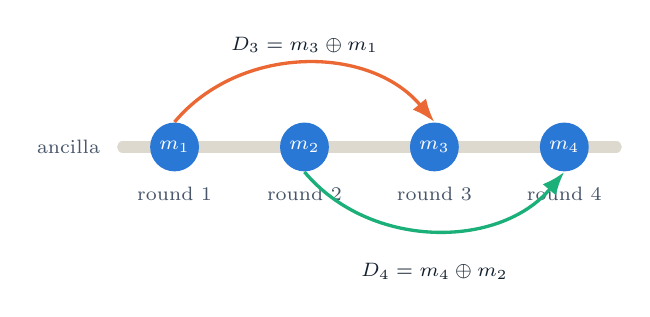
\begin{tikzpicture}[x=1.65cm,y=1cm,
  m/.style={circle,fill=cblue,text=white,inner sep=1.5pt,font=\scriptsize\bfseries,minimum size=0.62cm},
  s/.style={font=\scriptsize,color=soft}]
  \draw[gridc,line width=4pt,cap=round] (0.6,0) -- (4.4,0);
  \node[s,anchor=east] at (0.5,0) {ancilla};
  \foreach \k in {1,2,3,4} \node[m] (m\k) at (\k,0) {$m_\k$};
  \foreach \k in {1,2,3,4} \node[s] at (\k,-0.6) {round \k};
  \draw[corange,line width=1.2pt,-{Latex}] (m1.north) to[bend left=50] node[above,font=\scriptsize,color=ink]{$D_3 = m_3\oplus m_1$} (m3.north);
  \draw[caqua,line width=1.2pt,-{Latex}] (m2.south) to[bend right=50] node[below=8pt,font=\scriptsize,color=ink]{$D_4 = m_4\oplus m_2$} (m4.south);
\end{tikzpicture}
\end{column}
\begin{column}{0.5\textwidth}
\small
\textbf{With reset:} \quad $m_k = s_k$, \quad $D_k = m_k \oplus m_{k-1}$\\[6pt]
\textbf{Without reset (Emerald):}
\[ m_k = s_k \oplus m_{k-1} \;\Rightarrow\; s_k = m_k \oplus m_{k-1} \]
\[ D_k = s_k \oplus s_{k-1} = \boxed{m_k \oplus m_{k-2}} \]
{\color{soft}\footnotesize A detector still asks: did this stabilizer change between two rounds?}
\end{column}
\end{columns}
\vfill
\begin{beamercolorbox}[rounded=true,sep=6pt]{normal text}
\footnotesize \textbf{Implementation:} Stim's \texttt{MR}$\rightarrow$\texttt{M}; every \texttt{DETECTOR}/\texttt{OBSERVABLE} rewritten ($m_0=m_{-1}=0$; final data readout compared with $m_{\text{last}}\oplus m_{\text{last}-1}$).
\textbf{Check:} without noise, every detector is 0 in Stim and in Qiskit Aer.
\end{beamercolorbox}
\end{frame}

% ─────────────────────────────────────────────────────────────────────────────
\begin{frame}{Zero SWAPs, proven on the instructions sent to the QPU}
\eyebrow{2 \textperiodcentered\ Placement and compilation}
\begin{columns}[c]
\begin{column}{0.40\textwidth}
\centering
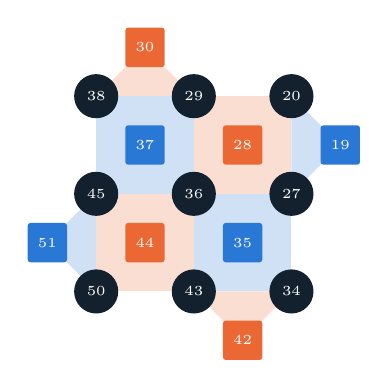
\begin{tikzpicture}[scale=0.62,
  dataq/.style={circle,fill=ink,text=white,inner sep=0pt,minimum size=0.56cm},
  ancz/.style={rectangle,rounded corners=1pt,fill=cblue,text=white,inner sep=0pt,minimum size=0.5cm},
  ancx/.style={rectangle,rounded corners=1pt,fill=corange,text=white,inner sep=0pt,minimum size=0.5cm}]
  \fill[xstab] (3.0,-1.0) -- (1.0,-1.0) -- (2.0,-0.0) -- cycle;
\fill[zstab] (1.0,-1.0) -- (3.0,-1.0) -- (3.0,-3.0) -- (1.0,-3.0) -- cycle;
\fill[xstab] (3.0,-1.0) -- (5.0,-1.0) -- (5.0,-3.0) -- (3.0,-3.0) -- cycle;
\fill[zstab] (5.0,-1.0) -- (5.0,-3.0) -- (6.0,-2.0) -- cycle;
\fill[zstab] (1.0,-3.0) -- (1.0,-5.0) -- (0.0,-4.0) -- cycle;
\fill[xstab] (1.0,-3.0) -- (3.0,-3.0) -- (3.0,-5.0) -- (1.0,-5.0) -- cycle;
\fill[zstab] (3.0,-3.0) -- (5.0,-3.0) -- (5.0,-5.0) -- (3.0,-5.0) -- cycle;
\fill[xstab] (3.0,-5.0) -- (5.0,-5.0) -- (4.0,-6.0) -- cycle;
\node[dataq] at (1.0,-1.0) {\tiny 38};
\node[dataq] at (3.0,-1.0) {\tiny 29};
\node[dataq] at (5.0,-1.0) {\tiny 20};
\node[dataq] at (1.0,-3.0) {\tiny 45};
\node[dataq] at (3.0,-3.0) {\tiny 36};
\node[dataq] at (5.0,-3.0) {\tiny 27};
\node[dataq] at (1.0,-5.0) {\tiny 50};
\node[dataq] at (3.0,-5.0) {\tiny 43};
\node[dataq] at (5.0,-5.0) {\tiny 34};
\node[ancx] at (2.0,-0.0) {\tiny 30};
\node[ancz] at (2.0,-2.0) {\tiny 37};
\node[ancx] at (4.0,-2.0) {\tiny 28};
\node[ancz] at (6.0,-2.0) {\tiny 19};
\node[ancz] at (0.0,-4.0) {\tiny 51};
\node[ancx] at (2.0,-4.0) {\tiny 44};
\node[ancz] at (4.0,-4.0) {\tiny 35};
\node[ancx] at (4.0,-6.0) {\tiny 42};

\end{tikzpicture}\\[2pt]
{\scriptsize\color{soft} Placement used (numbers = Emerald QB index). Circles: data; {\color{cblue}$\blacksquare$} Z and {\color{corange}$\blacksquare$} X ancillas. QB26 excluded.}
\end{column}
\begin{column}{0.58\textwidth}
\begin{tikzpicture}
\begin{axis}[deck, xbar, height=0.42\textheight, width=0.82\linewidth, xmin=0, xmax=290,
  symbolic y coords={ours,default,naive}, ytick={ours,default,naive},
  yticklabels={Ours, Qiskit default, Naive},
  y tick label style={font=\scriptsize,color=ink,align=right}, bar width=9pt,
  xlabel={CZ gates, $d=3$, 3 rounds}, grid=none, axis x line*=bottom, axis y line*=left,
  nodes near coords, nodes near coords style={font=\scriptsize,color=ink,anchor=west}]
  \addplot[fill=cgray,draw=none,bar shift=0pt] coordinates {(222,naive) (72,default)};
  \addplot[fill=cblue,draw=none,bar shift=0pt] coordinates {(72,ours)};
\end{axis}
\end{tikzpicture}
{\scriptsize
\begin{tabular}{@{}lll@{}}
Naive & 222 CZ, $\approx$\,50 SWAPs & \\
Qiskit default & 72 CZ, 0 SWAP & sim.\ $P_L$ 21.8\,\% (uses QB26)\\
\textbf{Ours} & \textbf{72 CZ, 0 SWAP} & \textbf{sim.\ $P_L$ 17.1\,\%}
\end{tabular}}\\[4pt]
{\scriptsize\color{soft} 76 zero-SWAP embeddings found by subgraph matching, all simulated in 5\,s. Transpiled with routing disabled; checked before every job: no SWAP, every CZ on a coupler in IQM's serialized instructions, every measurement in the right classical bit.}
\end{column}
\end{columns}
\end{frame}

% ─────────────────────────────────────────────────────────────────────────────
\begin{frame}{A known-state test before spending QPU time}
\eyebrow{3 \textperiodcentered\ Hardware check first}
\vspace*{0.6em}
\begin{columns}[T]
\begin{column}{0.24\textwidth}\bignum{17/17}{qubits return the expected bits through the full data path}\end{column}
\begin{column}{0.24\textwidth}\bignum{$\leq$1\,\%}{read 1 when prepared in $|0\rangle$}\end{column}
\begin{column}{0.24\textwidth}\bignum{\color{accent}2--15\,\%}{read 0 when prepared in $|1\rangle$: one-sided readout errors}\end{column}
\begin{column}{0.24\textwidth}\bignum{\color{accent}14$\rightarrow$39\,\%}{QB33 in $|1\rangle$ reads 0 at its 1st, then 2nd measurement}\end{column}
\end{columns}
\vfill
{\small The readout knocks qubits out of $|1\rangle$. Without reset this matters: an ancilla carries its measured state into the next round.}
\vspace*{1em}
\end{frame}

% ─────────────────────────────────────────────────────────────────────────────
\begin{frame}{Only the characterized noise model matches what Emerald does}
\eyebrow{4 \textperiodcentered\ Noise model: calibration, then characterization}
\begin{columns}[T]
\begin{column}{0.36\textwidth}\footnotesize
\textbf{Calibration model.} IQM per-qubit / per-coupler data (CZ 99.75\,\%, readout 99.68\,\%, $T_1\approx50\,\mu$s), depolarizing gates, $T_1/T_2$ idling sized by layer durations.\\[6pt]
\textbf{Characterization.} One error multiplier per qubit, fitted so the model reproduces the edge probabilities $p_{ij}$ measured from detector correlations (training shots). Typical factor $\times 2.1$.\\[6pt]
{\color{soft}\scriptsize Same circuit and decoder. Calibration: $\approx 4\times$ too optimistic; characterized: within 3--7\,\%.}
\end{column}
\begin{column}{0.62\textwidth}
\begin{tikzpicture}
\begin{axis}[deck, height=0.7\textheight, xlabel={QEC rounds}, ylabel={$P_L$ (\%), MWPM}, xtick={1,...,5},
  ymin=0, ymax=32, legend pos=north west]
  \addplot[caqua,dashed,mark=*] table[x=r,y=uniform] {data/sim_models.dat};
  \addlegendentry{Uniform 0.3\,\% (sim.)}
  \addplot[cblue,dashed,mark=*] table[x=r,y=calibrated] {data/sim_models.dat};
  \addlegendentry{IQM calibration (sim.)}
  \addplot[corange,dashed,mark=*] table[x=r,y=characterized] {data/sim_models.dat};
  \addlegendentry{Characterized (sim.)}
  \addplot[ink,mark=square*,error bars/.cd,y dir=both,y explicit] table[x=r,y=hardware,y error=hwerr] {data/sim_models.dat};
  \addlegendentry{Emerald, measured}
\end{axis}
\end{tikzpicture}
\end{column}
\end{columns}
\end{frame}

% ─────────────────────────────────────────────────────────────────────────────
{\setbeamercolor{background canvas}{bg=ink}\setbeamercolor{normal text}{fg=paper}\setbeamercolor{frametitle}{fg=paper}
\begin{frame}{What the syndromes revealed}
\color{paper}\eyebrow{5 \textperiodcentered\ A broken qubit the calibration cannot see}
\begin{columns}[c]
\begin{column}{0.45\textwidth}
{\Large\bfseries The calibration rated QB26 among the best qubits.\\[4pt] {\color{accent!80!white}Its own readout scrambles it.}}\\[10pt]
{\small\color{panel} Calibration: readout 99.8\,\%, $T_1 = 71\,\mu$s. Our characterization flagged it as the worst qubit ($\times 87$).\\[4pt]
Consequence: every MWPM variant did worse than no correction (3 rounds: 19.9\,\% $\rightarrow$ 27.3\,\%).}
\end{column}
\begin{column}{0.53\textwidth}
\begin{tikzpicture}
\begin{axis}[deck, height=0.62\textheight, xlabel={round}, ylabel={reads 1 (\%)}, xtick={1,...,5},
  ymin=0, ymax=60, tick label style={color=panel,font=\scriptsize}, label style={color=panel,font=\footnotesize},
  legend style={text=paper,at={(0.95,0.55)},anchor=east}, major grid style={ink!70!paper}, axis line style={ink!60!paper}]
  \addplot[corange!85!white,mark=*] coordinates {(1,8.2) (2,52.9) (3,50.0) (4,50.2) (5,49.3)};
  \addlegendentry{QB26 (Z ancilla)}
  \addplot[cblue!70!white,mark=*] coordinates {(1,2.3) (2,7.7) (3,10.1) (4,16.0) (5,18.8)};
  \addlegendentry{QB44 (Z ancilla, normal)}
  \draw[paper!60!ink,dashed] (axis cs:0.8,50) -- (axis cs:5.2,50);
  \node[font=\scriptsize,color=panel,anchor=south east] at (axis cs:4.6,52) {50\,\% = pure noise};
\end{axis}
\end{tikzpicture}
\end{column}
\end{columns}
\end{frame}}

% ─────────────────────────────────────────────────────────────────────────────
\begin{frame}{On the QPU: with QB26 decoding hurts; without it decoding wins}
\eyebrow{6 \textperiodcentered\ The fix, on hardware}
\begin{columns}[T]
\begin{column}{0.64\textwidth}
\begin{tikzpicture}
\begin{axis}[deck, height=0.72\textheight, xlabel={QEC rounds}, ylabel={$P_L$ (\%), held-out shots}, xtick={1,...,5},
  ymin=0, ymax=37, height=0.6\textheight, legend columns=2, legend style={at={(0.5,-0.3)},anchor=north,/tikz/every even column/.append style={column sep=8pt}}]
  \addplot[cgray,dashed,mark=*,error bars/.cd,y dir=both,y explicit] table[x=r,y=oldraw,y error=oldraw_e] {data/qpu.dat};
  \addlegendentry{With QB26, no correction}
  \addplot[corange,mark=*,error bars/.cd,y dir=both,y explicit] table[x=r,y=oldmw,y error=oldmw_e] {data/qpu.dat};
  \addlegendentry{With QB26, MWPM}
  \addplot[soft,dashed,mark=square*,error bars/.cd,y dir=both,y explicit] table[x=r,y=newraw,y error=newraw_e] {data/qpu.dat};
  \addlegendentry{QB26 excluded, no correction}
  \addplot[cblue,mark=square*,error bars/.cd,y dir=both,y explicit] table[x=r,y=newmw,y error=newmw_e] {data/qpu.dat};
  \addlegendentry{QB26 excluded, MWPM}
\end{axis}
\end{tikzpicture}
\end{column}
\begin{column}{0.33\textwidth}
\bignum{$-46$\,\%}{logical errors at 2 rounds, MWPM vs no correction, QB26 excluded}\\[14pt]
\bignum{12}{zero-SWAP placements left without QB26 (of 76)}\\[10pt]
{\scriptsize\color{soft} 400\,000 shots in total (100k with QB26, 300k without); 1$\sigma$ error bars.}
\end{column}
\end{columns}
\end{frame}

% ─────────────────────────────────────────────────────────────────────────────
\begin{frame}{Four decoders on the same hardware shots}
\eyebrow{7 \textperiodcentered\ MWPM, Union-Find, BP+OSD, GNN}
\centering
{\small
\begin{tabular}{@{}l S[table-format=2.1] S[table-format=2.1] S[table-format=2.1] S[table-format=2.1] S[table-format=2.1]@{}}
\toprule
Rounds & {No correction} & {MWPM} & {Union-Find} & {BP+OSD} & {GNN (defect graph)\unskip} \\
\midrule
\tableinput{data/decoders_table.tex}
\bottomrule
\end{tabular}}\\[10pt]
\begin{minipage}{0.92\linewidth}\scriptsize\color{soft}
$P_L$ in \%, 30k held-out shots per round count ($\pm$0.25\,\%); $\varepsilon_L$ in \% per round from the fit over rounds 2--5.
Union-Find: our weighted implementation (\texttt{ldpc}'s was worse than no correction in simulation).
BP+OSD on the full DEM hypergraph. GNN: next slide.
\end{minipage}
\end{frame}

% ─────────────────────────────────────────────────────────────────────────────
\begin{frame}{The GNN: a graph of the defects, learned on hardware shots}
\eyebrow{7 \textperiodcentered\ GNN architecture and variants}
\begin{columns}[T]
\begin{column}{0.55\textwidth}
\centering
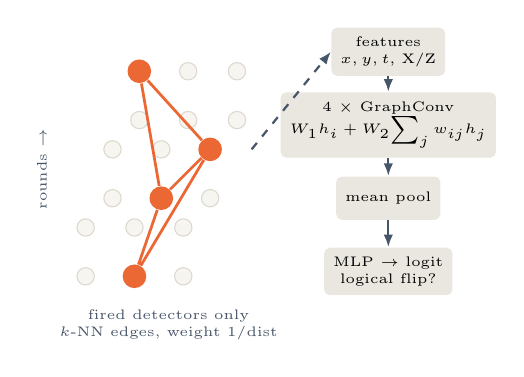
\begin{tikzpicture}[x=0.62cm,y=0.62cm,
  det/.style={circle,draw=gridc,fill=paper,inner sep=0pt,minimum size=0.22cm},
  fired/.style={circle,fill=corange,inner sep=0pt,minimum size=0.3cm},
  lay/.style={fill=panel,rounded corners=2pt,minimum width=1.25cm,minimum height=0.55cm,font=\tiny,align=center},
  arr/.style={-{Latex[length=1.6mm]},line width=0.8pt,color=soft}]
  % space-time detector lattice (3 rounds) with fired detectors
  \foreach \t in {0,1,2} {
    \foreach \x in {0,1,2} \foreach \y in {0,1} \node[det] at (\x+0.55*\t, \y+1.6*\t) {};
  }
  \node[fired] (f1) at (1+0.55*0, 0) {};
  \node[fired] (f2) at (2+0.55*1, 1+1.6) {};
  \node[fired] (f3) at (1+0.55*1, 0+1.6) {};
  \node[fired] (f4) at (0+0.55*2, 1+3.2) {};
  \draw[corange,line width=1pt] (f1) -- (f3) -- (f2) (f3) -- (f4) (f2) -- (f4) (f1) -- (f2);
  \node[font=\tiny,color=soft,align=center] at (1.7,-1.0) {fired detectors only\\ $k$-NN edges, weight $1/\text{dist}$};
  \node[font=\tiny,color=soft,rotate=90] at (-0.9,2.2) {rounds $\rightarrow$};
  % network
  \node[lay] (in) at (6.2,4.6) {features\\$x,y,t$, X/Z};
  \node[lay] (g) at (6.2,3.1) {4 $\times$ GraphConv\\$W_1h_i+W_2\!\sum_j w_{ij}h_j$};
  \node[lay] (p) at (6.2,1.6) {mean pool};
  \node[lay] (o) at (6.2,0.1) {MLP $\rightarrow$ logit\\logical flip?};
  \draw[arr] (in) -- (g); \draw[arr] (g) -- (p); \draw[arr] (p) -- (o);
  \draw[arr,dashed] (3.4,2.6) -- (in.west);
\end{tikzpicture}\\[2pt]
{\scriptsize\color{soft} Graph classification. Pre-trained on 60k simulated shots, fine-tuned on the hardware training half.}
\end{column}
\begin{column}{0.43\textwidth}
{\scriptsize
\begin{tabular}{@{}p{3.6cm}cc@{}}
\toprule
Variant & \multicolumn{2}{c}{$P_L$ (\%)}\\
 & 2 rounds & 3 rounds\\
\midrule
\tableinput{data/gnn_variants.tex}
\midrule
No correction & 15.0 & 23.0\\
MWPM & 8.2 & 16.3\\
\bottomrule
\end{tabular}}\\[6pt]
{\scriptsize\color{soft} Plain GCN (no time feature) fails at 3 rounds.}
\end{column}
\end{columns}
\end{frame}

% ─────────────────────────────────────────────────────────────────────────────
\begin{frame}{Bad-qubit exclusion matters more than the decoder}
\eyebrow{7 \textperiodcentered\ Exclusion $\times$ decoder (hardware)}
\begin{tikzpicture}
\begin{groupplot}[group style={group size=2 by 1,horizontal sep=1.2cm},
  deck, width=0.5\linewidth, height=0.62\textheight, ybar=1pt, /pgf/bar width=7pt, ymin=0, ymax=31,
  xtick={0,...,4}, xticklabels={No corr.,MWPM,UF,BP+OSD,GNN}, x tick label style={font=\scriptsize,color=ink},
  enlarge x limits=0.13, grid=none, ymajorgrids, legend style={at={(0.02,0.98)},anchor=north west},
  ]
\nextgroupplot[title={\footnotesize 2 rounds}, ylabel={$P_L$ (\%)}]
  \addplot[fill=corange,draw=none] table[x=i,y=old] {data/exclusion_r2.dat}; \addlegendentry{With QB26}
  \addplot[fill=cblue,draw=none] table[x=i,y=new] {data/exclusion_r2.dat}; \addlegendentry{QB26 excluded}
\nextgroupplot[title={\footnotesize 3 rounds}]
  \addplot[fill=corange,draw=none] table[x=i,y=old] {data/exclusion_r3.dat};
  \addplot[fill=cblue,draw=none] table[x=i,y=new] {data/exclusion_r3.dat};
\end{groupplot}
\end{tikzpicture}\\
{\scriptsize\color{soft} With QB26 every classical decoder is worse than no correction; the GNN (fixed-graph version here), trained on hardware shots, learns to ignore the scrambled ancilla (11.5\,\% at 2 rounds).}
\end{frame}

% ─────────────────────────────────────────────────────────────────────────────
\begin{frame}{The GNN found the broken qubit by itself}
\eyebrow{7 \textperiodcentered\ Ablation: scramble one ancilla, count changed decisions}
\begin{columns}[T]
\begin{column}{0.60\textwidth}
\begin{tikzpicture}
\begin{axis}[deck, height=0.70\textheight, ybar=2pt, /pgf/bar width=11pt, ymin=0, ymax=29,
  xtick={0,...,3}, xticklabels={QB10,QB26,QB28,QB44}, x tick label style={font=\footnotesize,color=ink},
  enlarge x limits=0.18, grid=none, ymajorgrids, ylabel={decisions changed (\%)},
  legend style={at={(0.02,0.98)},anchor=north west},
  nodes near coords={\pgfmathprintnumber[fixed,precision=0]{\pgfplotspointmeta}},
  every node near coord/.append style={font=\tiny,color=soft}]
  \addplot[fill=cblue,draw=none] table[x=i,y=mwpm] {data/ablation.dat}; \addlegendentry{MWPM}
  \addplot[fill=corange,draw=none] table[x=i,y=gnn] {data/ablation.dat}; \addlegendentry{GNN}
  \draw[accent,line width=1pt] (axis cs:0.62,-0.6) rectangle (axis cs:1.38,17.5);
\end{axis}
\end{tikzpicture}
\end{column}
\begin{column}{0.38\textwidth}\footnotesize
Hardware run \emph{with} QB26, 2 rounds, 15\,000 test shots. One Z ancilla's detectors are shuffled across shots: same firing rate, no information.\\[5pt]
\textbf{MWPM} trusts QB26: 15\,\% of its decisions change and its $P_L$ \emph{drops} ($17.7\rightarrow17.1\,\%$). QB26's syndrome is pure noise.\\[5pt]
\textbf{GNN}: only 5\,\% change. From shots alone it learned to lean on QB28 instead.\\[5pt]
{\scriptsize\color{soft} X ancillas do not touch the Z observable. The GNN also leans less on QB10, which shares data qubits with QB28.}
\end{column}
\end{columns}
\end{frame}

% ─────────────────────────────────────────────────────────────────────────────
\begin{frame}{From error probability to error rate per round}
\eyebrow{8 \textperiodcentered\ Fit over round counts}
\begin{columns}[T]
\begin{column}{0.62\textwidth}
\begin{tikzpicture}
\begin{axis}[deck, height=0.72\textheight, xlabel={QEC rounds $n$}, ylabel={$P_L$ (\%), hardware}, xtick={2,...,5},
  ymin=0, ymax=37, xmin=1.5, xmax=5.5, legend pos=north west]
  \addplot[cgray,mark=none] table[x=n,y=raw] {data/fitcurves.dat}; \addlegendentry{No correction}
  \addplot[cblue,mark=none] table[x=n,y=mwpm] {data/fitcurves.dat}; \addlegendentry{MWPM}
  \addplot[corange,mark=none] table[x=n,y=gnn] {data/fitcurves.dat}; \addlegendentry{GNN}
  \addplot[cgray,only marks,mark=*] table[x=r,y=raw] {data/decoders.dat};
  \addplot[cblue,only marks,mark=*] table[x=r,y=mwpm] {data/decoders.dat};
  \addplot[corange,only marks,mark=*] table[x=r,y=gnn] {data/decoders.dat};
\end{axis}
\end{tikzpicture}
\end{column}
\begin{column}{0.36\textwidth}\small
\[ 2P_L(n) = 1 - A\,(1-2\varepsilon_L)^n \]
\textbf{MWPM: $\varepsilon_L = 9.8 \pm 0.1\,\%$ / round}\\
{\color{soft}\footnotesize No correction 11.5\,\%; Union-Find 9.5\,\%; BP+OSD 10.0\,\%.}\\[8pt]
{\footnotesize $A$ absorbs state preparation and final readout. The README form ($A=1$) fits poorly: the error per round \emph{grows} with depth, $\approx$4.3\,\% at 2 rounds $\rightarrow$ 7.7\,\% at 5. Ancillas that are never reset accumulate damage.}
\end{column}
\end{columns}
\end{frame}

% ─────────────────────────────────────────────────────────────────────────────
\begin{frame}{Threshold: the curves cross at $\approx 0.45\times$ Emerald's noise}
\eyebrow{9 \textperiodcentered\ Simulation with the characterized model}
\begin{columns}[T]
\begin{column}{0.64\textwidth}
\begin{tikzpicture}
\begin{axis}[deck, height=0.72\textheight, xmode=log, ymode=log, log basis x=10,
  xlabel={physical noise relative to Emerald today}, ylabel={$\varepsilon_L$ (\% / round, rounds $=d$)},
  xtick={0.2,0.3,0.4,0.5,0.6,0.8,1}, xticklabels={0.2,0.3,0.4,0.5,0.6,0.8,1},
  legend pos=north west, log ticks with fixed point]
  \addplot[cblue,mark=*] table[x=f,y=d3] {data/threshold.dat}; \addlegendentry{$d=3$}
  \addplot[corange,mark=*] table[x=f,y=d5] {data/threshold.dat}; \addlegendentry{$d=5$}
  \addplot[caqua,mark=*] table[x=f,y=d7] {data/threshold.dat}; \addlegendentry{$d=7$}
  \draw[soft,dashed] (axis cs:1,0.05) -- (axis cs:1,20);
  \node[font=\scriptsize,color=soft,anchor=south east] at (axis cs:0.98,0.07) {Emerald today};
\end{axis}
\end{tikzpicture}
\end{column}
\begin{column}{0.34\textwidth}\small
Below the crossing, a larger code protects better; above it, a larger code is worse.\\[8pt]
{\color{soft}\footnotesize Larger patches do not fit on Emerald: each qubit's noise is drawn from Emerald's measured spread. A projection from a model validated at $d=3$; leakage and failures like QB26 are not modelled.}
\end{column}
\end{columns}
\end{frame}

% ─────────────────────────────────────────────────────────────────────────────
\begin{frame}{Logical error rate vs distance}
\eyebrow{9 \textperiodcentered\ Projection: today, $\div 2$, $\div 4$ noise}
\begin{columns}[T]
\begin{column}{0.62\textwidth}
\begin{tikzpicture}
\begin{axis}[deck, height=0.72\textheight, ymode=log, xtick={3,5,7}, xticklabels={$d=3$,$d=5$,$d=7$},
  ylabel={$\varepsilon_L$ (\% / round)}, xmin=2.6, xmax=7.4, legend pos=south west, log ticks with fixed point]
  \addplot[cblue,mark=*] table[x=d,y=today] {data/distance.dat}; \addlegendentry{Emerald today}
  \addplot[corange,mark=*] table[x=d,y=half] {data/distance.dat}; \addlegendentry{noise $\div 2$}
  \addplot[caqua,mark=*] table[x=d,y=quarter] {data/distance.dat}; \addlegendentry{noise $\div 4$}
\end{axis}
\end{tikzpicture}
\end{column}
\begin{column}{0.36\textwidth}\small
\[\Lambda = \varepsilon_L(d)/\varepsilon_L(d+2)\]
\begin{tabular}{@{}lcc@{}}
\toprule
Noise & $\Lambda_{3\to5}$ & $\Lambda_{5\to7}$\\
\midrule
today & 0.76 & 0.97\\
$\div 2$ & 1.04 & 1.13\\
$\div 4$ & \textbf{1.97} & \textbf{2.00}\\
\bottomrule
\end{tabular}\\[8pt]
{\footnotesize\color{soft} At a quarter of today's noise each $+2$ in distance halves $\varepsilon_L$, the level Google reported with Willow.}
\end{column}
\end{columns}
\end{frame}

% ─────────────────────────────────────────────────────────────────────────────
{\setbeamercolor{background canvas}{bg=ink}\setbeamercolor{normal text}{fg=paper}\setbeamercolor{frametitle}{fg=paper}
\begin{frame}{What we built, found and measured}
\color{paper}\eyebrow{Takeaways}
\begin{columns}[T]
\begin{column}{0.31\textwidth}
{\color{accent!80!white}\Large\bfseries Built}\\[4pt]
{\small\color{panel} A no-reset $d=3$ surface code on Emerald with zero SWAPs proven, a calibrated and characterized noise model, and four decoders, all validated on hardware.}
\end{column}
\begin{column}{0.31\textwidth}
{\color{accent!80!white}\Large\bfseries Found}\\[4pt]
{\small\color{panel} Calibration misses what limits the code: QB26 scrambled by its own readout, and ancilla errors that depend on their last result. Only the syndromes show it, and a GNN trained on them learns to distrust QB26 on its own.}
\end{column}
\begin{column}{0.31\textwidth}
{\color{accent!80!white}\Large\bfseries Measured}\\[4pt]
{\small\color{panel} $\varepsilon_L\approx$ 9.5--10\,\% per round across four decoders; up to $-55$\,\% logical errors vs no correction (GNN, 2 rounds). Threshold at $\approx0.45\times$ today's noise.}
\end{column}
\end{columns}
\vfill
{\footnotesize\color{panel} Next: leakage- and history-aware decoding, dynamical decoupling during readout, the X basis.}
\vspace*{1em}
\end{frame}}

\end{document}
